\chapter{算法理论推导与 MATLAB 仿真}
\label{chap:algorithm}

\section{算法流程与成像坐标约定}
本章从相机成像模型出发，推导镜头去畸变、姿态矫正及自适应 Gamma 校正算法，
并给出图像重采样与 MATLAB 仿真的组织方法。
其中，去畸变处理镜头引入的非线性几何误差，姿态矫正处理相机旋转导致的投影变化，
Gamma 校正调整像素亮度映射。前两者共同确定输出像素在源图像中的位置，
后者作用于像素值，三者的处理对象和评价方法有所区别。

本系统在源图像上执行自适应 Gamma，再通过组合几何映射一次性完成姿态与镜头补偿，
最后重采样得到输出图像。将两个几何变换合并，可以避免依次生成中间图像造成的重复插值。
Gamma 是非线性变换，通常不满足“先插值后增强”与“先增强后插值”等价，
仿真与后续硬件比较时应保持处理顺序一致。

\subsection{针孔模型与内参矩阵}
设相机坐标系中空间点为 $(X_c,Y_c,Z_c)$，归一化成像坐标为
\begin{equation}
x=\frac{X_c}{Z_c},\qquad y=\frac{Y_c}{Z_c}.
\end{equation}
忽略像素轴倾斜时，理想像素坐标 $(u,v)$ 满足
\begin{equation}
\lambda\begin{bmatrix}u\\v\\1\end{bmatrix}
=K\begin{bmatrix}X_c\\Y_c\\Z_c\end{bmatrix},\qquad
K=\begin{bmatrix}f_x&0&c_x\\0&f_y&c_y\\0&0&1\end{bmatrix},
\label{eq:camera-intrinsics}
\end{equation}
其中 $f_x,f_y$ 为以像素计的焦距，$c_x,c_y$ 为主点坐标。
本章采用列向量表示；原仿真使用的 MATLAB \path{cameraParameters.IntrinsicMatrix}
为该矩阵的转置，读取时需显式转换。

\subsection{标定数据与像素中心}
算法采用以下相机标定参数：
\begin{equation}
K=\begin{bmatrix}
748.4469&0&944.9033\\
0&748.0773&522.3963\\
0&0&1
\end{bmatrix}.
\end{equation}
\begin{equation}
(k_1,k_2)=(0.0099,-0.0434),\qquad(p_1,p_2)=(0,0).
\end{equation}
这些参数记录于原仿真的 \path{para.txt}，与 FPGA 工程中的标定记录一致。
输入与输出图像均为 $1920\times1080$，采用相同内参和尺寸。
图像裁切或缩放时，主点与焦距按像素变换关系相应调整。

MATLAB 图像的像素中心从 1 开始，列坐标对应 $u$，行坐标对应 $v$，
数组访问顺序为 $I(v,u)$。因此输出视线为
\begin{equation}
\boldsymbol d_o=K^{-1}[u,v,1]^{\mathsf T}
=\left[\frac{u-c_x}{f_x},\frac{v-c_y}{f_y},1\right]^{\mathsf T}.
\end{equation}
FPGA 接口使用从 0 开始的坐标，建立视线时应先加 1，最终源像素坐标再减 1。
这一转换改变的是像素索引约定，不应通过修改标定焦距进行补偿。

\section{镜头去畸变算法}
\subsection{径向与切向畸变模型}
镜头畸变描述理想视线与实际感光平面位置之间的偏差。
设归一化理想坐标为 $(x,y)$，到主点的归一化距离平方为
\begin{equation}
r^2=x^2+y^2.
\end{equation}
二阶径向畸变模型取到 $r^4$ 项，径向缩放系数为
\begin{equation}
L(r)=1+k_1r^2+k_2r^4.
\end{equation}
切向畸变常用于描述镜片与成像平面不完全平行等偏心因素，
将两者叠加可得
\begin{align}
x_d&=xL(r)+2p_1xy+p_2(r^2+2x^2),\label{eq:distort-x}\\
y_d&=yL(r)+p_1(r^2+2y^2)+2p_2xy.\label{eq:distort-y}
\end{align}
畸变源图像中的像素位置为
\begin{equation}
u_s=f_xx_d+c_x,\qquad v_s=f_yy_d+c_y.
\label{eq:distort-pixel}
\end{equation}
所用标定中 $p_1=p_2=0$，仍在程序中保留完整切向项，
并以非零参数和已知坐标进行公式检查，避免零系数掩盖实现错误。

\subsection{由正向成像模型构造逆映射}
若逐个源像素寻找矫正后位置，非整数投影和离散取整可能导致多个源像素落入同一位置，
也可能使部分输出位置无人写入。输出驱动的逆映射则遍历每个理想输出像素，
用式~\eqref{eq:distort-x}--\eqref{eq:distort-pixel} 直接计算它对应的畸变源坐标：
\begin{equation}
I_o(u,v)=\mathcal S\left(I_s,\,u_s(u,v),\,v_s(u,v)\right),
\end{equation}
其中 $\mathcal S$ 为重采样算子。
这里不必逐像素求解畸变多项式的反函数，因为已知的是理想输出位置，
实际需要的是该视线在原始畸变图像中的位置。

映射坐标应保留符号与小数精度，先进行有效性判断，再转换为数组索引。
参考实现用双精度坐标图保存 $u_s,v_s$，将无效位置标为非数值，
避免负坐标转换为无符号整数后回绕到图像另一侧。

\subsection{去畸变 MATLAB 仿真}
仿真程序使用 \path{cameraParameters} 建立相机模型，
将内置 \path{undistortImage} 与按式~\eqref{eq:distort-x}、
式~\eqref{eq:distort-y} 构造的映射进行比较。
映射、采样和实验入口分别封装，统一使用相同标定与边界规则。
\path{run_undistort_simulation.m} 读取同一张真实相机图像，
分别生成浮点双线性、5 位权重双线性和最近邻结果，
记录有效区域比例及量化误差。
若安装 Computer Vision Toolbox，则额外调用内置去畸变函数，
并用 \path{undistortPoints} 检查稀疏映射点的反向坐标一致性。
内置图像的输出原点也会保存，避免不同输出视场之间直接做像素相减。

\begin{figure}[htbp]
\centering
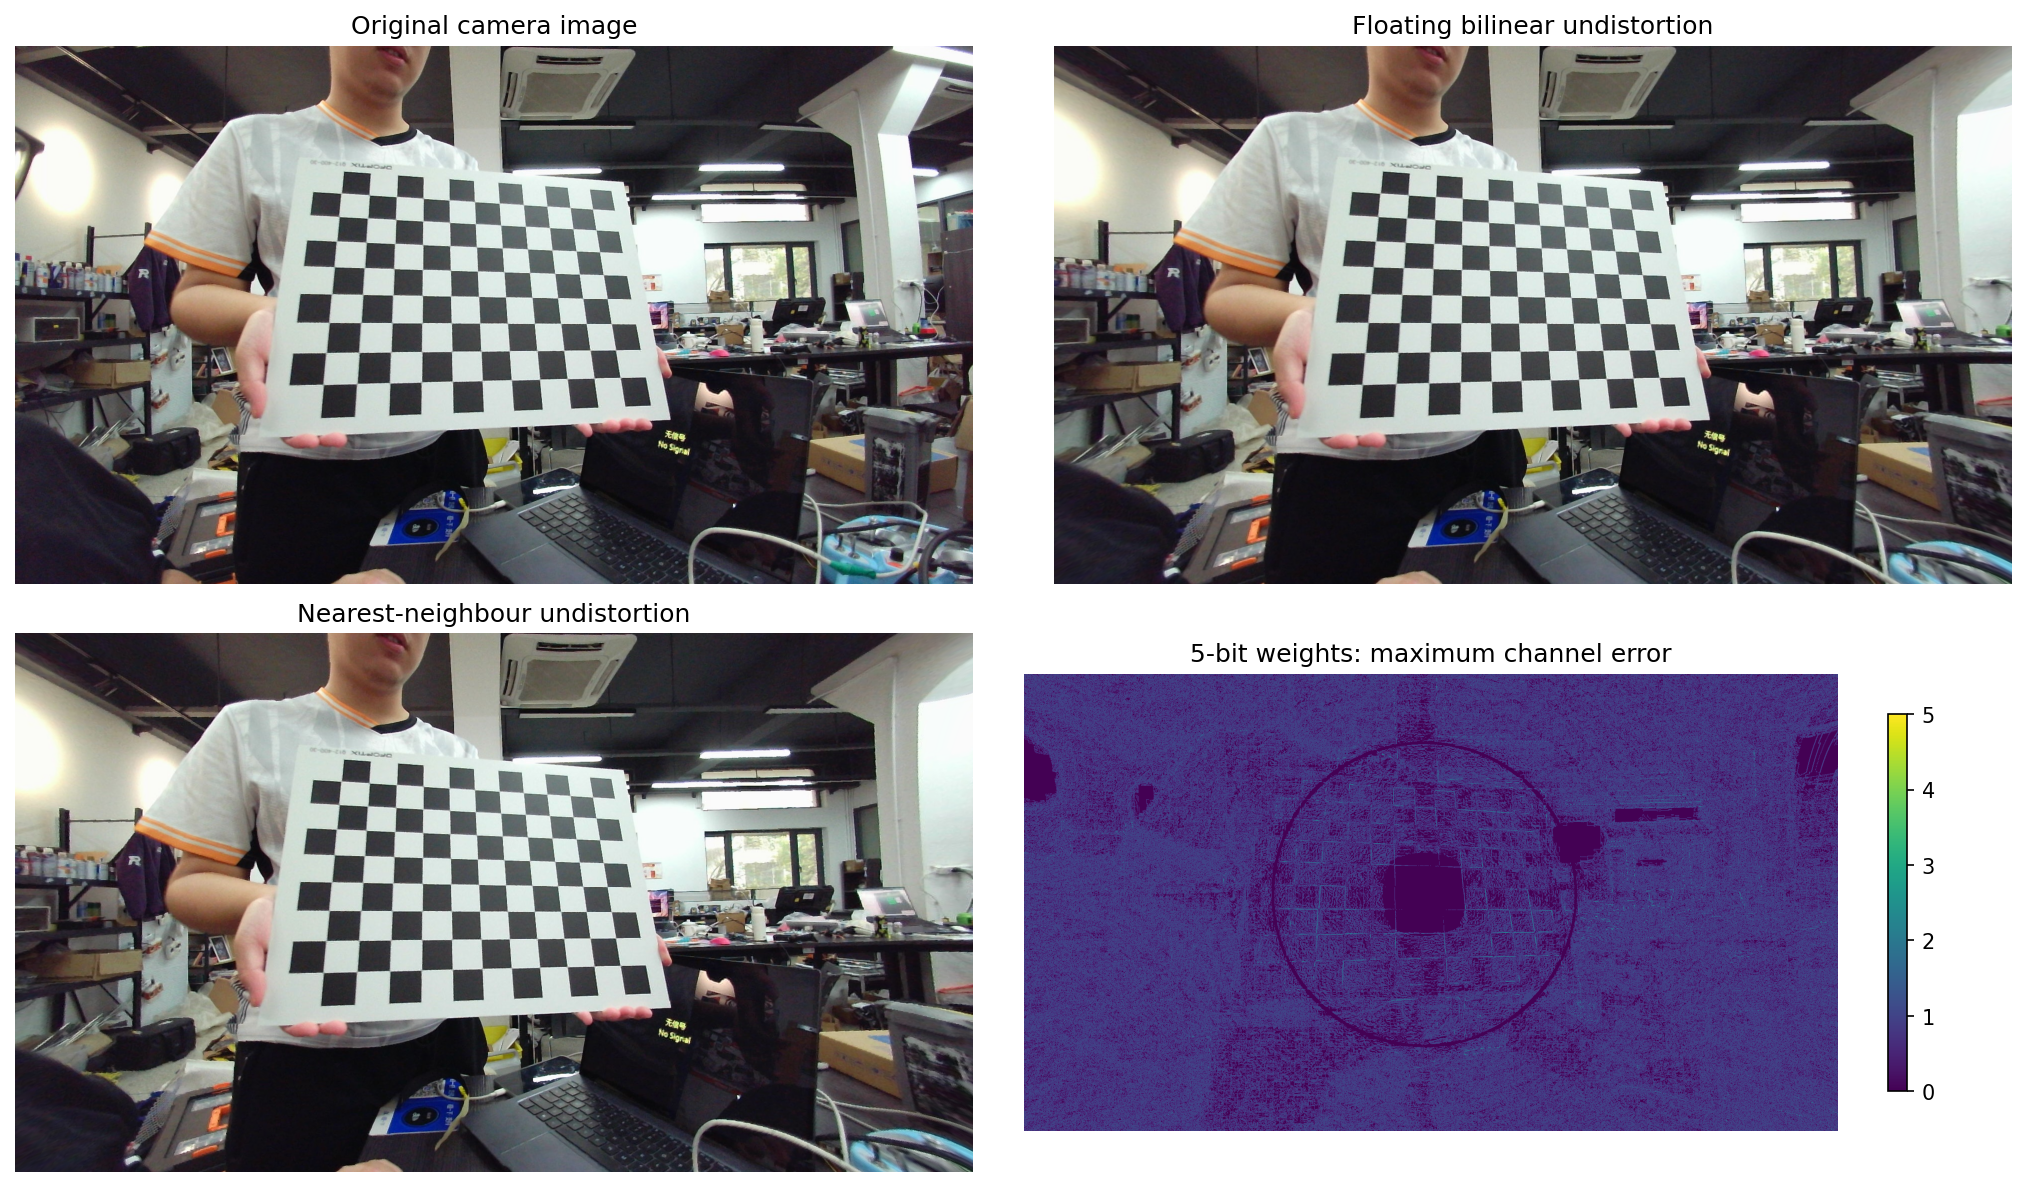
\includegraphics[width=\textwidth]{chapter3/figures/undistort_comparison_reference.png}
\caption{真实相机图像的去畸变与插值对比（独立数值交叉检查生成）}
\label{fig:undistort-simulation}
\end{figure}

\section{姿态矫正算法}
\subsection{参考视线到源相机视线的变换}
镜头去畸变并不能消除相机方向变化引起的透视变化，
因此还需建立参考视场与当前相机视场之间的旋转关系。
本章定义相机坐标轴为 $x$ 向右、$y$ 向下、$z$ 向前，
以 yaw 角 $\psi$ 和 pitch 角 $\theta$ 描述工程使用的两个姿态自由度。
相应旋转矩阵为
\begin{equation}
R_y(\psi)=\begin{bmatrix}
\cos\psi&0&\sin\psi\\0&1&0\\-\sin\psi&0&\cos\psi
\end{bmatrix},\qquad
R_x(\theta)=\begin{bmatrix}
1&0&0\\0&\cos\theta&-\sin\theta\\0&\sin\theta&\cos\theta
\end{bmatrix}.
\end{equation}
按实际算法的运算顺序，输出参考视线先进行 yaw 变换，再进行 pitch 变换，故
\begin{equation}
\boldsymbol d_s=R\boldsymbol d_o,\qquad R=R_x(\theta)R_y(\psi).
\label{eq:pose-rotation}
\end{equation}
若 $C$ 表示源相机坐标到参考坐标的姿态矩阵，则
$C=R^{\mathsf T}=R_y(-\psi)R_x(-\theta)$。
区分 $C$ 与 $R$ 可以避免将相机物理旋转直接当作逆采样方向。

令 $\boldsymbol d_o=[x,y,1]^{\mathsf T}$，先计算
\begin{align}
X_1&=\cos\psi\,x+\sin\psi,&Y_1&=y,&Z_1&=-\sin\psi\,x+\cos\psi,
\end{align}
再计算
\begin{align}
X_s&=X_1,\\
Y_s&=\cos\theta\,Y_1-\sin\theta\,Z_1,\\
Z_s&=\sin\theta\,Y_1+\cos\theta\,Z_1.
\end{align}
透视归一化后的源相机理想坐标为
\begin{equation}
x_s=X_s/Z_s,\qquad y_s=Y_s/Z_s.
\label{eq:pose-normalize}
\end{equation}
当 $Z_s$ 接近零或为负时，视线不具备稳定的前向投影，应判为无效。

\subsection{单应关系与姿态、镜头补偿的组合}
仅考虑相机绕光心旋转且暂不考虑镜头畸变时，有
\begin{equation}
\lambda\boldsymbol p_s=H\boldsymbol p_o,\qquad
H=K_sRK_o^{-1}.
\label{eq:pose-homography}
\end{equation}
本系统中 $K_s=K_o=K$。由于存在齐次除法，yaw/pitch 引起的变换一般是投影变换，
不能直接用二维平移或一般仿射近似替代整个视场的映射。
纯旋转模型不依赖场景深度；如果云台转轴偏离光心而产生明显平移，
不同深度目标会出现视差，该模型无法同时消除所有视差。

组合补偿的计算顺序为
\begin{equation}
\boldsymbol p_o\ \xrightarrow{K_o^{-1}}\ \boldsymbol d_o
\ \xrightarrow{R}\ \boldsymbol d_s
\ \xrightarrow{\text{透视归一化}}\ (x_s,y_s)
\ \xrightarrow{\text{镜头模型}}\ (x_d,y_d)
\ \xrightarrow{K_s}\ (u_s,v_s).
\end{equation}
即将式~\eqref{eq:pose-normalize} 的结果代入镜头模型，最后只进行一次图像重采样。
这也说明不能直接在畸变像素平面上套用理想相机的单应矩阵。

\subsection{姿态输入、有效域与 MATLAB 实验}
工程姿态量按每弧度 2048 个整数单位传送，解码关系为
\begin{equation}
\psi=q_\psi/2048,\qquad\theta=q_\theta/2048.
\end{equation}
当前 FPGA 分块通路的每轴限幅约为 $\pm15^\circ$，roll 不参与变换。
MATLAB 使用双精度三角函数，并单独比较角度量化前后的坐标，
用以分析姿态输入量化误差；它并未模拟 RTL 的每一级截断和查表误差。

\path{run_pose_simulation.m} 构造已知的彩色网格参考平面，
先用 $R^{\mathsf T}$ 合成当前相机图像，再用 $R$ 进行矫正。
该实验关闭镜头畸变以单独考察旋转关系，测试零姿态、单轴转动、双轴组合及边界角度。
理论检查将程序得到的源坐标经式~\eqref{eq:pose-homography} 的逆变换投回，
统计与原输出坐标的差异；图像检查则统计两次采样后与参考图的 RGB 误差。
两者分别反映几何一致性和离散重采样损失，不能混为同一精度指标。

\begin{figure}[htbp]
\centering
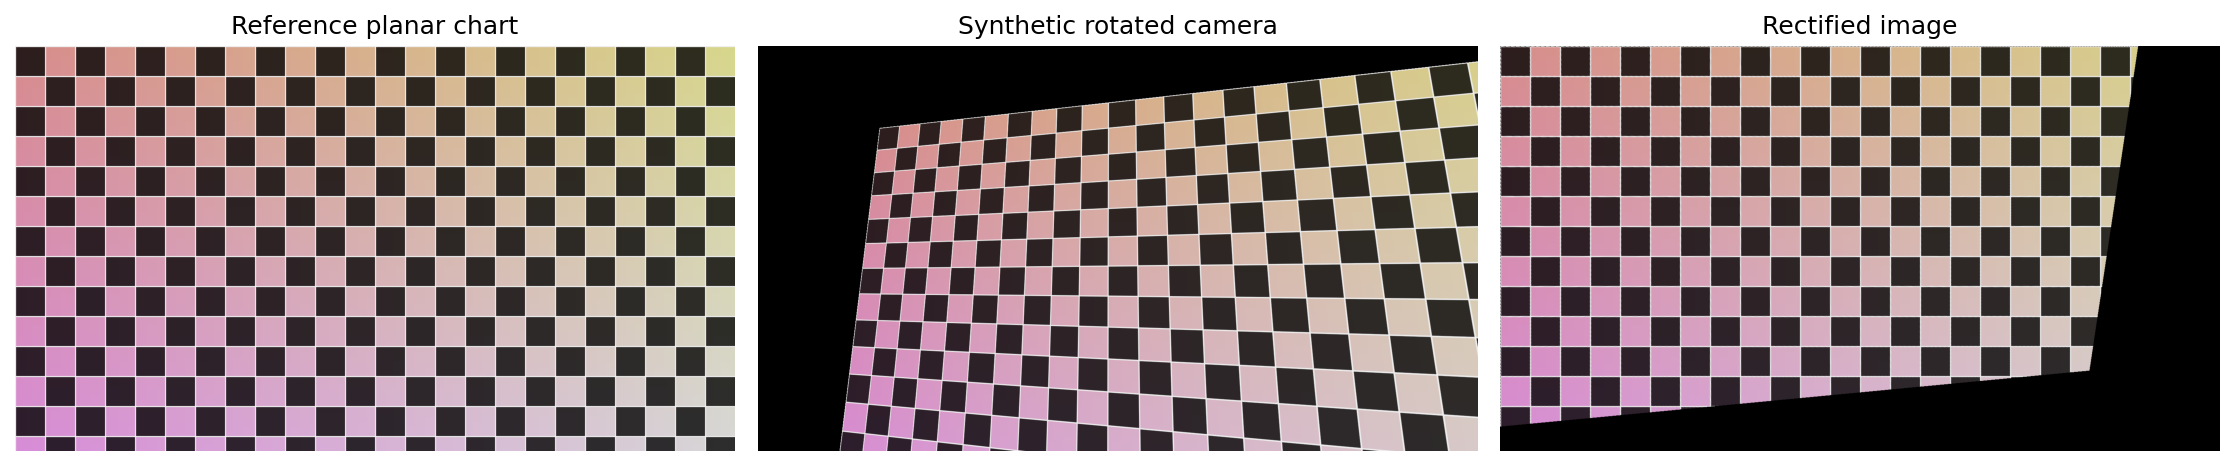
\includegraphics[width=\textwidth]{chapter3/figures/pose_correction_reference.png}
\caption{已知参考网格、合成相机图像与姿态矫正结果（独立数值交叉检查生成）}
\label{fig:pose-simulation}
\end{figure}

统计图像误差时，仅使用输入与合成图像共同可见、且四个插值邻点均有效的区域。
视场外像素置黑，不能把填黑区域当作真实图像参与误差评价。
这类合成实验验证数学映射关系，物理云台的轴向、IMU 零点与时间同步仍需单独实测。

\section{图像重采样及通用处理方法}
\subsection{最近邻与双线性插值}
源坐标 $(u_s,v_s)$ 通常不是整数。最近邻采样选择最近像素，
\begin{equation}
I_o(u,v)=I_s\left(\left\lfloor u_s+\tfrac12\right\rfloor,
\left\lfloor v_s+\tfrac12\right\rfloor\right),
\end{equation}
上式采用图像坐标书写，程序数组索引仍为先行后列。
最近邻实现简单、读取次数少，但会在斜边与细纹理处产生明显的锯齿或跳变。

双线性插值先沿水平方向对相邻两个像素作线性插值，再沿竖直方向插值。
设 $i=\lfloor u_s\rfloor$、$j=\lfloor v_s\rfloor$，
$\alpha=u_s-i$、$\beta=v_s-j$，则
\begin{align}
I_o={}&(1-\alpha)(1-\beta)I_s(i,j)
+\alpha(1-\beta)I_s(i+1,j)\notag\\
&+(1-\alpha)\beta I_s(i,j+1)
+\alpha\beta I_s(i+1,j+1).
\label{eq:bilinear}
\end{align}
四个权重非负且和为 1，因此常值图像应保持不变，线性灰度平面在内部区域可以精确重建。
双线性插值能改善局部连续性，但也可能使高频细节变软，
其效果应结合斜边和纹理区域评价，不能仅凭观感认定清晰度提高。

\subsection{权重量化与整数累加}
为研究有限精度影响，设置 $F=2^b$，将小数位置量化为
\begin{equation}
a=\operatorname{round}(F\alpha),\qquad
b_q=\operatorname{round}(F\beta).
\end{equation}
将式~\eqref{eq:bilinear} 的四个权重改写为整数乘积，先计算
\begin{align}
A={}&(F-a)(F-b_q)I_{00}+a(F-b_q)I_{10}\notag\\
&+(F-a)b_qI_{01}+ab_qI_{11},
\end{align}
再取 $I_o=\lfloor A/F^2\rfloor$。
原仿真使用 $b=5$，故最后除以 $2^{10}$ 可由移位完成。
量化值允许等于 $F$，因此权重在程序中不能被误当作只能表示 $0\ldots F-1$ 的整数。
仿真还保留浮点权重并在输出处取整的参考路径，二者差异包含权重量化和最终舍入规则的影响。

\subsection{边界、有效掩码与颜色处理}
对不在源图像闭区间 $[1,W]\times[1,H]$ 内的坐标，默认输出黑色并记录无效掩码。
对恰好位于末行或末列的有效坐标，重复边界邻点完成退化的一维插值，
从而保证零变换可以完整保留原图。另提供边界复制模式用于方案比较，
但该模式会把边缘内容延伸到视场外，不能视为恢复了未采集的信息。

有效掩码应来自映射与采样条件，不能根据输出 RGB 是否为零判断，
因为图像本身也可能包含黑色目标。
数值保护还限制相机后方视线及径向模型的过度外推。
共用参考函数的深度阈值取 $1024/2^{18}$，径向支持上限取 $r^2\leq600000/2^{18}$，
与工程数值保护保持联系；该上限是算法支持域，不代表独立测得的镜头视场。

RGB 三个通道使用同一组坐标和权重分别插值。
本章参考保留 RGB888，用于观察算法与采样误差；硬件帧缓存采用 RGB565，
比较硬件输出时还应单独考虑颜色量化。
误差统计统一限定到共同有效区域 $\Omega$，例如
\begin{equation}
E_{\rm RGB}=\sqrt{\frac{1}{3|\Omega|}
\sum_{(u,v)\in\Omega}\sum_{c\in\{R,G,B\}}
\left(I_o^{(c)}(u,v)-I_{\rm ref}^{(c)}(u,v)\right)^2}.
\end{equation}
几何坐标误差则以像素为单位，按二维坐标距离计算，不能与灰度级误差直接比较。

\section{帧自适应 Gamma 矫正算法}
\subsection{Gamma 变换与查找表}
将 8 位像素 $z$ 归一化为 $s=z/255$，本系统直接以指数 $\gamma$ 定义变换
\begin{equation}
T_\gamma(z)=\operatorname{round}\left[255\left(\frac{z}{255}\right)^\gamma\right].
\label{eq:gamma-transform}
\end{equation}
这里的指数就是 $\gamma$，没有另取其倒数。
当 $0<\gamma<1$ 时提升中低灰度，当 $\gamma>1$ 时压低中间灰度，
$\gamma=1$ 时保持恒等映射。端点 0 和 255 保持不变，映射单调，
但无法恢复曝光时已饱和或被噪声淹没的细节。

本系统设置七档指数
\begin{equation}
\gamma_c\in\{0.50,0.65,0.80,1.00,1.25,1.55,1.90\},
\qquad c=0,1,\ldots,6.
\end{equation}
每档预先生成 256 项查找表，RGB 三通道共用同一条曲线并独立查表。
对三个通道分别施加非线性变换仍可能改变通道比值和饱和度，
因此增强评价除平均亮度外还应观察颜色表现。

\begin{figure}[htbp]
\centering
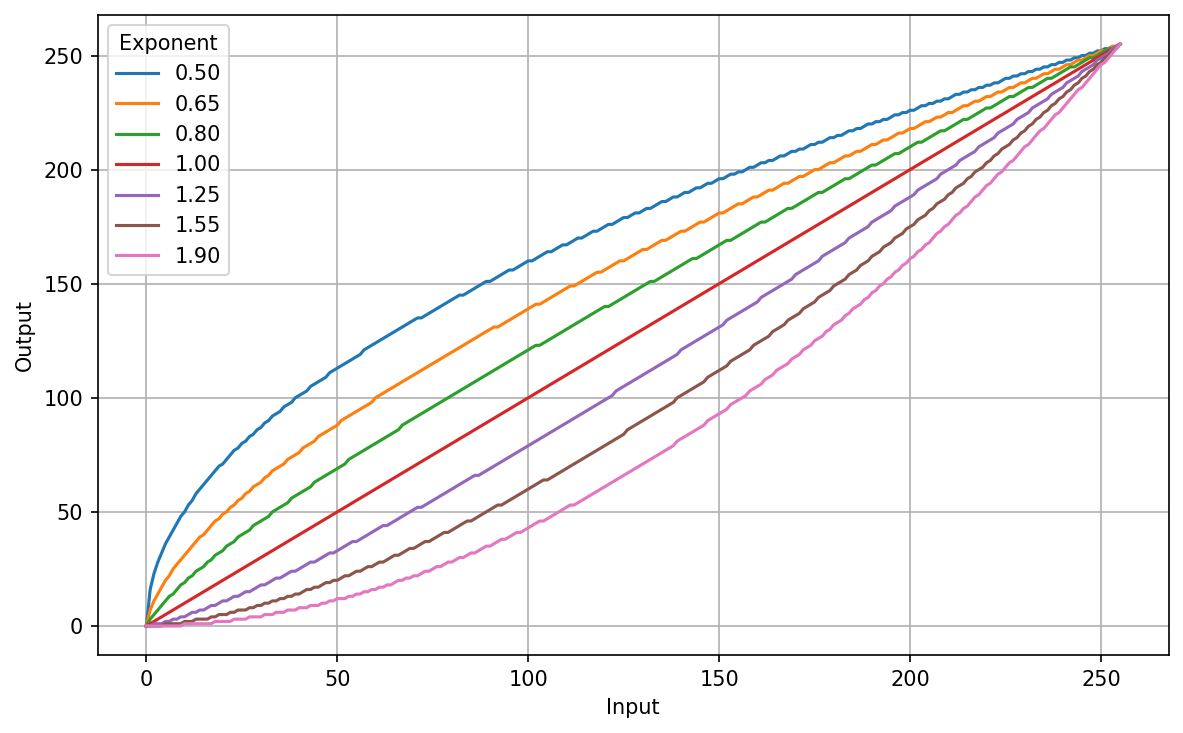
\includegraphics[width=0.76\textwidth]{chapter3/figures/gamma_curves_reference.png}
\caption{七档 Gamma 像素映射曲线（独立数值交叉检查生成）}
\label{fig:gamma-curves}
\end{figure}

\subsection{原始亮度统计与曲线选择}
为降低硬件统计代价，用整数近似亮度
\begin{equation}
Y=\left\lfloor\frac{R+2G+B}{4}\right\rfloor.
\end{equation}
只统计有效图像像素，定义帧像素数 $N$、亮度和 $S$、暗像素数 $D$ 和高光像素数 $H$：
\begin{equation}
S=\sum Y,\qquad D=\sum\mathbf1(Y<48),\qquad H=\sum\mathbf1(Y\geq208),
\qquad\mu=S/N.
\end{equation}
统计对象始终为增强前的原始输入，避免输出亮度改变后反过来驱动选档而形成振荡。
若 $D/N\geq1/8$ 且 $H/N\geq1/8$，优先判为混合光照，选择 $c=2$，
采用温和的暗部提升；否则按表~\ref{tab:gamma-classification} 选择候选曲线。

\begin{table}[htbp]\centering\small
\caption{非混合光照场景的 Gamma 选档规则}
\label{tab:gamma-classification}
\begin{tabular}{ccc}
\toprule
原始帧平均亮度 $\mu$ & 曲线编号 $c$ & 指数 $\gamma_c$\\
\midrule
$\mu<48$ & 0 & 0.50\\
$48\leq\mu<80$ & 1 & 0.65\\
$80\leq\mu<112$ & 2 & 0.80\\
$112\leq\mu\leq144$ & 3 & 1.00\\
$144<\mu\leq176$ & 4 & 1.25\\
$176<\mu\leq208$ & 5 & 1.55\\
$208<\mu$ & 6 & 1.90\\
\bottomrule
\end{tabular}
\end{table}

硬件中不必实际求平均值或比例，例如 $\mu<48$ 改写为 $S<48N$，
混合光照条件改写为 $8D\geq N$ 且 $8H\geq N$，
可利用常数乘法、移位和比较完成。

\subsection{跨帧确认与平滑切换}
为抑制图像内容变化带来的亮度闪烁，系统要求连续两帧得到相同候选分类后，
才更新目标曲线；实际曲线在每个帧起点最多向目标移动一档，且整帧固定。
令 $c_n$ 为第 $n$ 帧的候选分类，$a_n$ 为该帧使用的实际曲线，
$t_n$ 为第 $n$ 帧起点完成上一帧分类后的目标，则
\begin{align}
a_n&=a_{n-1}+\operatorname{sgn}(t_{n-1}-a_{n-1}),\\
t_n&=\begin{cases}
c_{n-1},&c_{n-1}=c_{n-2}\text{ 且两个分类均有效},\\
t_{n-1},&\text{其他情况}.
\end{cases}
\end{align}
初始实际曲线与目标曲线均为 3，即恒等映射。
第 $n-1$ 帧统计在第 $n$ 帧开始时才完整可用，
且该帧实际曲线已按旧目标锁定，新目标最早影响第 $n+1$ 帧。
例如从启动起连续输入暗图，前六帧实际曲线依次为 $3,3,3,2,1,0$。
MATLAB 模型保留这一因果顺序，不用当前帧的全图统计提前处理当前帧。

\subsection{自适应 Gamma MATLAB 仿真}
\path{run_gamma_simulation.m} 以真实图像为基础，构造正常、暗光、强光及左右混合光照
四种受控测试输入，每种连续输入 10 帧，记录原始与增强后平均亮度、候选、目标和实际曲线。
为减少实验开销，仅在这个无几何变换的实验中对图像作四倍间隔抽样。
这些输入用于测试响应机制，不等同于真实低照度传感器噪声或自动曝光过程。

\begin{figure}[htbp]
\centering
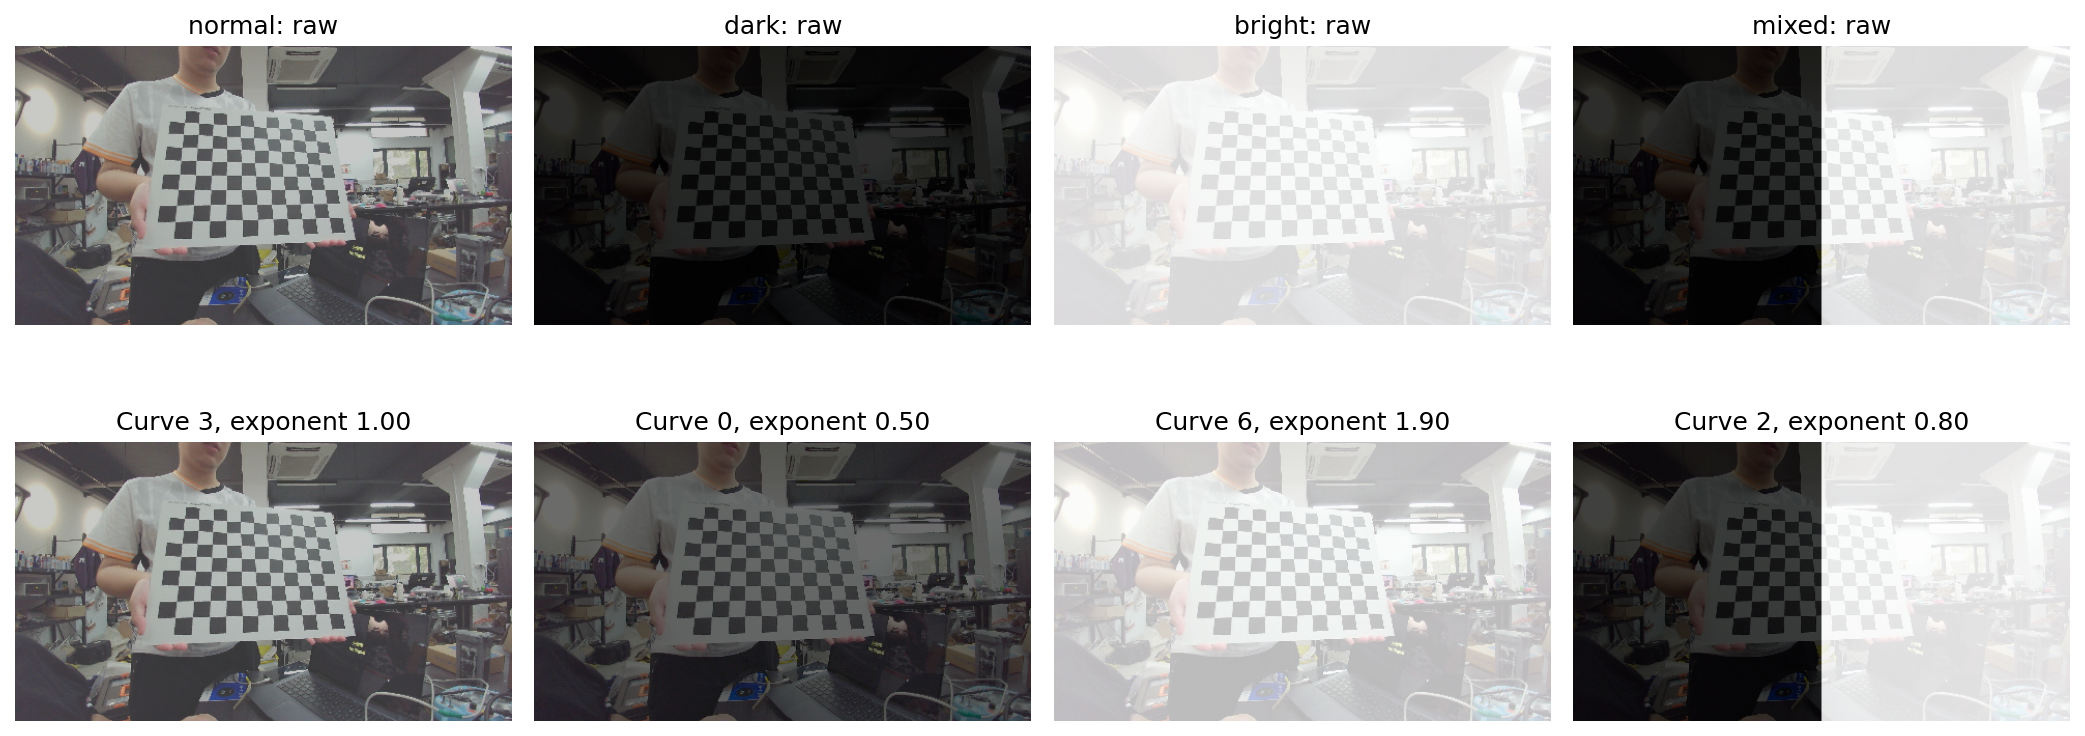
\includegraphics[width=\textwidth]{chapter3/figures/gamma_scenes_reference.png}
\caption{四种受控光照场景及稳定后的增强效果（独立数值交叉检查生成）}
\label{fig:gamma-scenes}
\end{figure}

\begin{figure}[htbp]
\centering
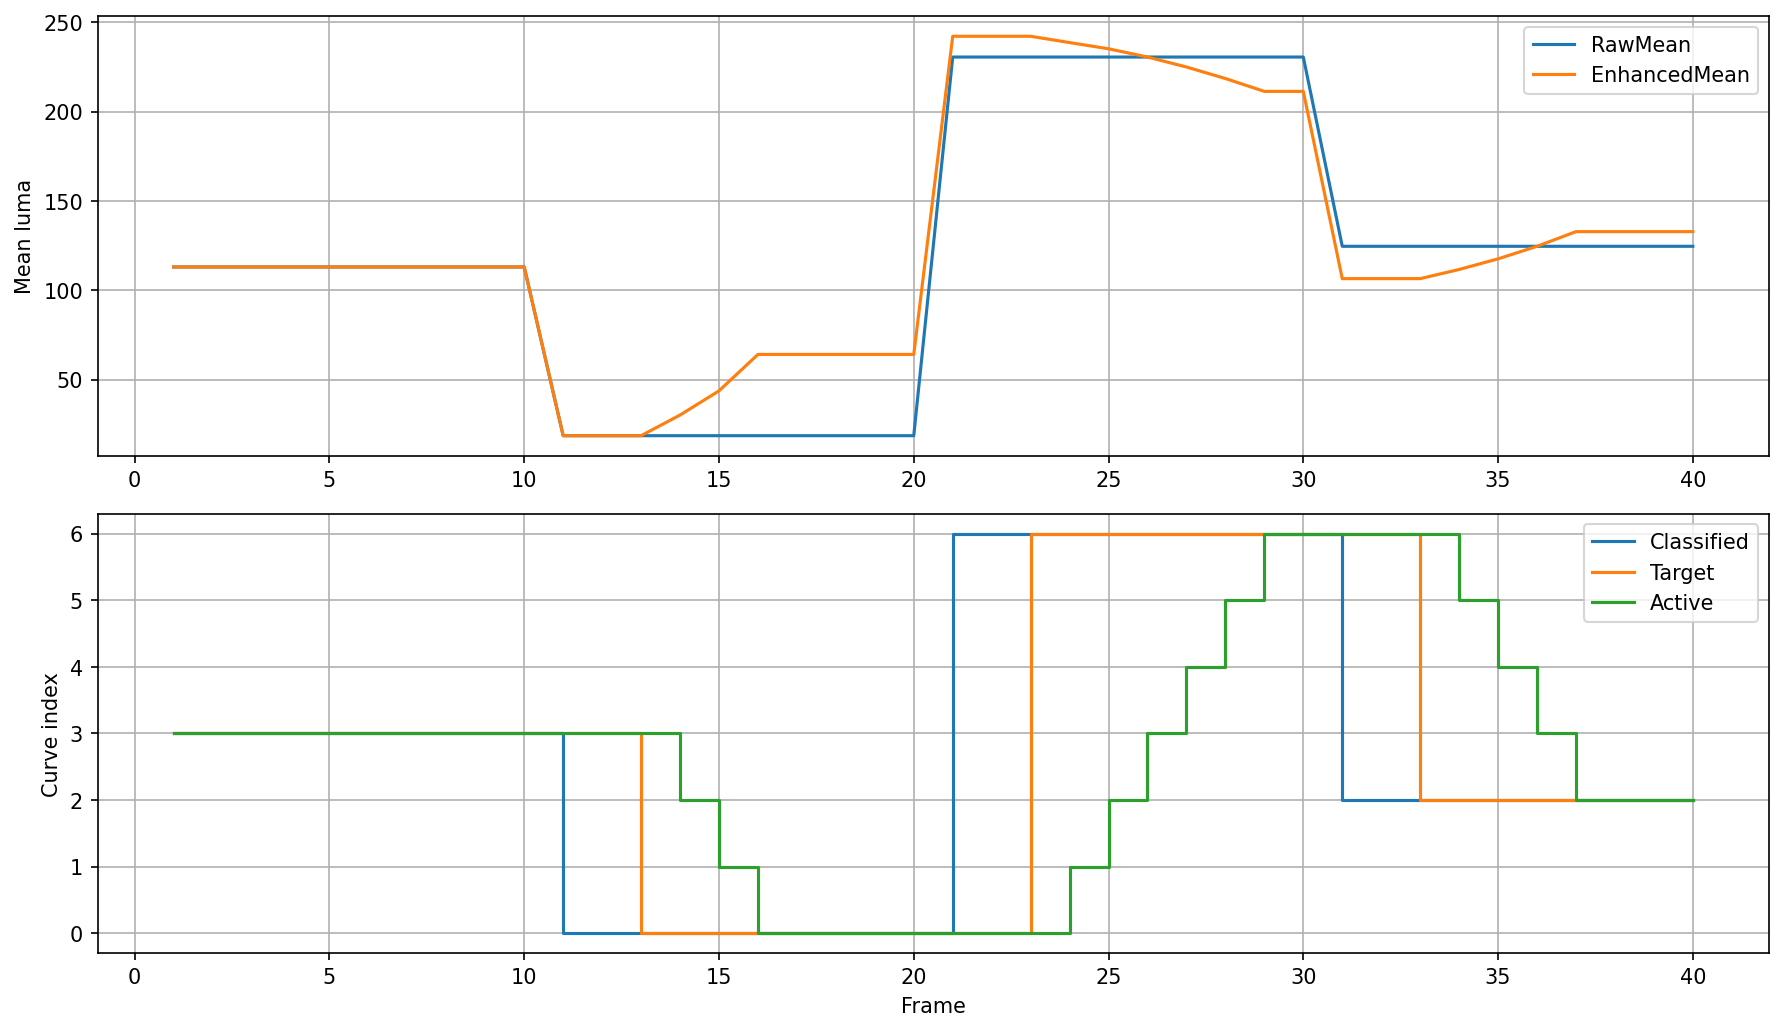
\includegraphics[width=0.9\textwidth]{chapter3/figures/gamma_transition_reference.png}
\caption{亮度统计与曲线切换的帧序列（独立数值交叉检查生成）}
\label{fig:gamma-transition}
\end{figure}

\section{仿真代码组织与结果分析}
\subsection{目录与复现入口}
所有 MATLAB 仿真位于 \path{chapter3/reference/}，
共用参数只在 \path{common/simulation_config.m} 中定义，主要文件见表~\ref{tab:matlab-files}。
输入图像与标定文本作为固定实验数据，计算结果保存于 \path{results/}，
报告插图保存于 \path{chapter3/figures/}。

\begin{table}[htbp]\centering\small
\caption{MATLAB 仿真程序组织}
\label{tab:matlab-files}
\begin{tabularx}{\textwidth}{>{\raggedright\arraybackslash}p{8.5cm}Y}
\toprule
文件（相对于 \path{chapter3/reference/}） & 功能\\
\midrule
\path{run_all_simulations.m} & 三个算法的统一运行入口\\
\path{check_simulation_models.m} & 解析样例、边界和控制时序检查\\
\path{common/inverse_camera_map.m} & 姿态与镜头模型的组合坐标映射\\
\path{common/sample_image.m} & 最近邻、浮点和量化双线性采样\\
\path{common/pose_rotation.m} & 姿态旋转矩阵\\
\path{common/adaptive_gamma_frame.m} & 带历史状态的因果帧级 Gamma 模型\\
\path{undistort/run_undistort_simulation.m} & 去畸变及插值精度比较\\
\path{pose/run_pose_simulation.m} & 合成图卡、姿态扫描及角度量化实验\\
\path{gamma/run_gamma_simulation.m} & 复杂光照与帧间响应实验\\
\bottomrule
\end{tabularx}
\end{table}

在报告根目录启动 MATLAB 后执行：
\begin{verbatim}
addpath('chapter3/reference');
run_all_simulations;
\end{verbatim}
核心算法只依赖 MATLAB 基础数组、图像读写和绘图功能；
内置去畸变比较需要 Computer Vision Toolbox，
保留的图卡质量评估函数还依赖 Image Processing Toolbox。
没有相应工具箱时，手工模型仍可运行，内置比较按可用性跳过。

\subsection{独立数值验证结果}
算法参考程序 \path{verify_reference.py} 使用 SciPy 插值和矩阵运算，
对几何映射、颜色重采样与 Gamma 控制关系进行独立数值验证。
本章图示与数值均来自该程序；MATLAB 程序提供同模型复现入口，
未列入已执行的 MATLAB 测试结果，数值验证也不作为 FPGA 实板测量。

在 $1920\times1080$ 测试图像上，零姿态去畸变映射的有效区域占比为 100\%，
该比例描述既定参数与输出视场下的坐标覆盖。
5 位权重双线性与浮点双线性的最大通道差为 5 灰度级，RGB 均方根差约为 0.677 灰度级。
该结果反映插值权重及取整差异，不能据此代替镜头标定精度或图像清晰度指标。

在 yaw 为 $10^\circ$、pitch 为 $-8^\circ$ 的合成图卡实验中，
共同有效区域约占 73.83\%，两次采样后的 RGB 均方根误差约为 8.88 灰度级。
六组姿态的连续坐标往返误差低于 $10^{-9}$ 像素，
而仅对输入角度作 Q2048 量化后，该双轴场景的源坐标均方根变化约为 0.239 像素。
这说明连续几何一致性、姿态量化和图像插值损失应分别评价。

在稳定后的暗光测试段，平均亮度从约 18.67 提升至 64.14；
强光段从约 230.51 降至 211.30；混合光照选择指数为 0.80 的温和曲线。
七档曲线及安全恒等档的 2048 项数值与 FPGA Gamma ROM 一致，
帧间实际曲线变化也满足每帧至多一档的约束。
这些结果验证了模型的数值关系与控制逻辑，最终画质、颜色、动态姿态同步及硬件吞吐
分别在后续硬件与测试章节中评价。
